%%%%%%%%%%%%%%%%%%%%%%%%%%%%%%%
%%% 第二章 基于深度学习的机械臂分拣系统设计
%%%%%%%%%%%%%%%%%%%%%%%%%%%%%%%

\chapter{基于深度学习的机械臂分拣系统设计}

自动分拣系统的核心为图像处理模块,该模块的核心为目标检测算法。传统的目标检测算法需要人为为工件构造特征,
通过模板匹配的方式确定工件位置,再通过分类器的方式确定工件类别。当变换检测工件时,就需要针对工件再次构造特征。
而基于深度学习的目标检测算法则可以实现端到端的训练。这使得基于深度学习的机械臂分拣系统具有很强的可移植性。

自动分拣系统是一个多模块协同作用的系统。包括图像采集模块、图像处理模块和机械臂控制模块。这三个模块均建立在硬件
基础之上,且需要高效的通信机制。本章主要介绍整个自动分拣系统的整体架构和底层设计,包括硬件选型、通信流程等。然后
介绍了如何选择本系统中使用的目标检测算法,至于具体模型的介绍、训练及部署等,将放到第三章去讨论。最后,本章将介绍
目前相对已经比较成熟的相机标定及机械臂控制方法。

\section{系统整体架构}

系统的逻辑层面的架构图如图    \ref{fig:total_construct}
所示。

\begin{figure}[htbp]
    \centering
    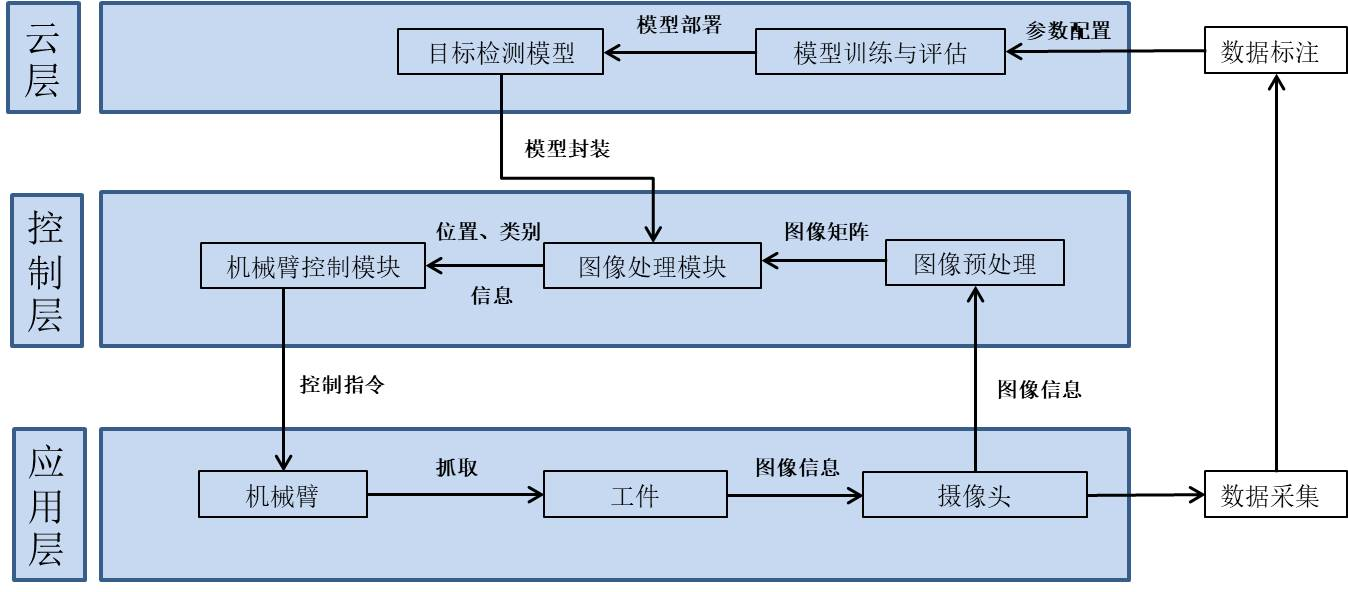
\includegraphics[width=\textwidth]{pic/chap2/total_construct.jpg}
    \caption{系统逻辑架构图}
    \label{fig:total_construct}
\end{figure}

基于深度学习的机械臂分拣系统逻辑上可以分为三个层面:应用层、控制层和云层(即服务器层)。以下对每个层面进行具体介绍:

1. 应用层

应用层由机械臂、工件和摄像头组成。主要是摄像头收集工件信息,机械臂对工件执行抓取动作。这一层面是整个系统对外展示的层面,
代表了整个系统的表现。

2. 控制层

控制层主要进行信息的处理和机械臂的控制指令生成。首先,控制层接收由应用层摄像头发送的图像信息,并进行预处理,之后发送给图像处理
模块中的目标检测模型进行预测,得到工件的位置和类别信息,然后发送给机械臂控制模块,由机械臂控制模块生成相应的机械臂控制指令,发送给
机械臂进行执行。

其中,摄像头和控制层的通信通过USB完成,所使用的摄像头为USB摄像头,主要是进行图像信息的传输;控制层和机械臂之间通过串口进行通信,
主要是进行机械臂控制指令的传输,如G代码等;而控制层的模块之间,则通过
机器人控制系统(Robot Operation System,ROS)进行,主要进行整型或浮点数的传输。

3. 云层(服务器层)

服务器层主要用于系统的搭建,在系统运行时是不参与工作的。服务器主要提供计算资源,用于深度学习模型的训练和评估。训练完成后,得到的其实是模型配置文件
和由大量浮点数组成的权重文件。模型配置文件主要用于描述模型的结构和参数,权重文件则用于描述模型网络的各个参数值。有了这些,就可以将模型部署和封装到
控制层,用于预测图像中工件的位置和信息。

此外,在三个层之外,还需要使用摄像头采集数据集,并进行标注,用作服务器层模型训练的数据集。

\section{系统硬件选型}

作为机械自动化及高性能计算一体的系统,基于深度学习的自动化分拣系统对硬件环境非常依赖。硬件性能的好坏将直接影响目标检测模型
的迭代次数、机械臂响应速度和分拣的延迟。因此,自动分拣系统的硬件选型非常重要。

本节主要介绍系统的硬件选型,包括用于采集图像信息的USB摄像头、用于高性能计算的服务器、运行图像处理模块和机械臂控制模块的
高性能嵌入式平台以及用于抓取工件的机械臂。

\subsection{相机}

\subsection{目标检测模型训练用服务器}

\subsection{目标检测运行硬件平台}

\subsection{机械臂选型}

\subsection{系统硬件架构}

\section{系统模块间通信机制}

\subsection{USB通信}

本系统中,USB通信主要用于摄像头向TX2传递图像信息。
本课题使用的USB版本为USB 3.0    \cite{USB3.0}版本,其传输速度为5Gbit/s,足以支撑高FPS的图像传输。

\subsection{ROS通信}

\subsection{串口通信}

\section{目标检测算法选型}

\section{相机标定及机械臂控制模块设计与实现}



